\documentclass{beamer}

\usepackage{alltt}
\usepackage[utf8]{inputenc}
\usepackage{qtree}

\title{Milner}
\author{Alan Hu}
\date{2020}

\begin{document}

\frame{\titlepage}

\begin{frame}[fragile]
  \frametitle{Milner}
  Over the past three weeks, I've been creating my own programming language,
  Milner

\begin{verbatim}
external puts : (Cstring) -> ()

val main : () -> Int32
fun main() =
  puts("Hello, world!");
  0i32
\end{verbatim}
\end{frame}

\begin{frame}
  \frametitle{What is a Programming Language?}
  \begin{itemize}
    \pause
  \item Syntax
    $$
    e ::= \lambda x.e \mid e(e) \mid x, y, z...
    $$
    \pause
  \item Semantics
    $$
    \frac{e_1 \longrightarrow e_1'}{e_1(e_2) \longrightarrow e_1'(e_2)}
    $$
    $$
    \frac{}{(\lambda x.e_1)(e_2) \longrightarrow e_1[x/e_2]}
    $$
  \end{itemize}
  \pause
  A programming language is an abstract idea
\end{frame}

\begin{frame}
  A programming language \textit{implementation} realizes the abstract language
  definition
  \begin{itemize}
    \pause
  \item Compiler
    \begin{itemize}
      \pause
      \item Translate source language into machine language (executable file)
    \end{itemize}
    \pause
  \item Interpreter
    \begin{itemize}
      \pause
    \item Execution is evaluation
    \end{itemize}
  \end{itemize}
  A \textit{reference implementation} is a specification for the language
\end{frame}

\begin{frame}
  \frametitle{Compilers}
  How does a compiler or interpreter work?
  \begin{itemize}
    \pause
  \item Lexer
    \pause
  \item Parser
    \pause
  \item Analysis
    \pause
  \item Codegen
  \end{itemize}
  \pause
  In practice, interpreters compile to a low-level \textit{bytecode} which is
  then executed
\end{frame}

\begin{frame}
  \begin{figure}
    
\includegraphics[scale=0.25]{ocaml-color-logo.png}
  \end{figure}
  \begin{itemize}
    \pause
  \item OCaml - Implementation language
    \pause
  \item Developed at Inria - Coq proof assistant as motivation
    \pause
  \item Descendant of Robin Milner's proof assistant meta language, ML
    \pause
  \item Excels at compiler development, symbolic manipulation
  \end{itemize}
\end{frame}

\begin{frame}
  \frametitle{Reading}
  Compilers aren't magical
  \begin{itemize}
    \pause
  \item A programming language is a file format
    \pause
  \item Read file, process data, output file
    \pause
  \item Compilers are glorified file converters
    \pause
  \item Files are sequences of bytes on your hard disk
    \pause
  \item Parse text into an abstract syntax tree
    \pause
  \item $1 + 2 \times 3$
    \pause
  \item \Tree [.add num(1) [.mul num(2) num(3) ] ]
  \end{itemize}
\end{frame}

\begin{frame}
  \begin{figure}
    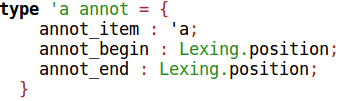
\includegraphics[scale=0.5]{ast-annot.png}
    \caption{Source location annotation}
  \end{figure}
  \begin{figure}
    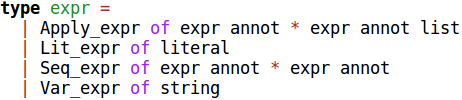
\includegraphics[scale=0.5]{ast-expr.png}
    \caption{Expression tree definition}
  \end{figure}
\end{frame}

\begin{frame}
  \frametitle{Typechecking}
  \begin{itemize}
    \pause
  \item Not all programs have a meaning
    \begin{itemize}
      \pause
    \item ``Hello'' + 1
      \pause
    \item True(3)
    \end{itemize}
  \item Ascribe a ``type'' to each term
    \pause
  \item Static semantics
    \begin{itemize}
      \pause
    \item
      $$
      \frac{e_1 : Int \quad e_2 : Int}{e_1 + e_2 : Int}
      $$
      \pause
    \item
      $$
      \frac{e_1 : A \to B \quad e_2 : A}{e_1 (e_2) : B}
      $$
    \end{itemize}
  \item Hindley-Milner type system
  \end{itemize}
\end{frame}

\begin{frame}
  \frametitle{Code Generation}
  \begin{itemize}
    \pause
  \item $M$ languages, $N$ target architectures
    \pause
  \item $M \times N$ compiler combinations
    \pause
  \item Separate compiler into \textit{frontend} and \textit{backend}
    \pause
  \item $frontend : Source \to IR$
    \pause
  \item $backend : IR \to Target$
    \pause
  \item $compiler : Source \to Target$
    \pause
  \item $compiler = backend \circ frontend$
  \end{itemize}
\end{frame}

\begin{frame}
  \frametitle{LLVM}
  \begin{figure}
    
\includegraphics[scale=0.5]{LLVM-Logo-Derivative-1.png}
  \end{figure}
  \begin{itemize}
    \pause
  \item LLVM - Low-Level Virtual Machine
    \pause
  \item SSA - Static Single Assignment
    \pause
  \item Official OCaml API - https://llvm.moe/
  \end{itemize}
\end{frame}

\begin{frame}[plain,c]
  \begin{center}
    \huge Questions?
  \end{center}
\end{frame}

\end{document}
